\section{A risk-based approach to the OTS}

\subsection{Grid designs and security}

The authors of \cite{eggletonNETWORKSTRUCTURESUBTRANSMISSION1993} expose various
designs of power grids and analyze the implications in terms of security level. Underlying
their rationale is the principle that the lower the consequences, the more
acceptable they are. By applying that logic, the distribution systems are
operated radially, though such an operating scheme puts all the connected users under
the risk of being shut down by the contingency of any element of the string of elements
connecting it to the source substation. In contrast, transmission systems dealing
with larger areas are exposed to bigger consequences and foster a meshed operation
to secure each substation. Therefore, the bulk transmission grid is operated fully
meshed, whereas underneath, subtransmission parts are operated looped or meshed,
some parts being operated as pocket under one single feeding point, or groups connected
to multiple feeding points.

These parts of the transmission grid are more prone to being operated with insecure
areas. This is especially the case where the grid is weakly developed, or if the
development could not follow the settlement of grid users, during maintenance
periods that require outages of nonredundant elements, or following a contingency.
One must accept that some areas of the system -- even if internally meshed --
would only be connected to the main part of the network through a single branch.
In that case, should this branch trip, the whole area is de-energized.

But that insecurity does not mean that the transmission system operator lacks control.
The consequences of each potential contingency must be clearly identified and
mastered. No tripping should result in violation of physical limits, cascading
effects, or grid collapses. Should a given contingency lead to loss of a part of
the system with loads and/or generations, the extent of the consequences must be
assessed \emph{a priori} and weighted against its probability of occurrence.

\subsection{Implication to the transmission switching design process}

This aspect of policy must be considered by operators when designing their
operational strategies and especially when designing the switching patterns. In that context, the risk of overloading a branch may be unacceptable. Indeed, even if the probability is low, the consequence is unacceptable as this could destroy assets or worse still expose people around to potentially fatal outcomes.

Consider the case of a subtransmission area connected to the bulk grid through two branches. Suppose that the tripping of one of both leads to an overloading of the other, so the operator must take a preventive action. One option consists in involving grid users in the area and requesting a change in their injections, which is costly, and would need to be done irrespective of whether the contingency occurs. The other consists in splitting the area into two disconnected pockets, each hanging on one branch. Now, if a tripping occurs on one of these branches, the corresponding pocket is lost, but there would be no forbidden overloading.
That is an application of the security/cost trade-off: to decide between spending money for redispatching and ensuring security or taking the risk of losing an area, which would be very unlikely, but with potential significantly higher costs. In the latter case, this may imply the search for an optimum among all the possibilities of splitting the area into two pockets. This is the focus of this paper.

\begin{figure}
    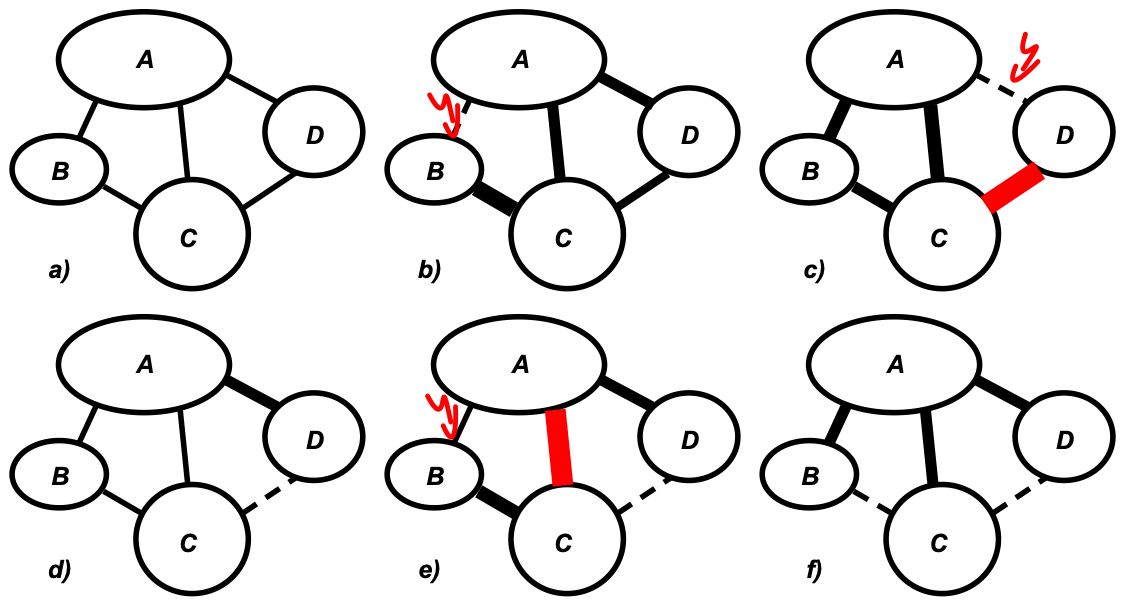
\includegraphics[width=\linewidth]{images/Un-meshing.png}
    \caption{Preventive-openings-cascade. Each bubble represents a portion of a grid a)
    the initial pattern; b) after the tripping of $AB$, no overload and B is secured; c) the tripping of $AC$ result in an overload on $CD$ which implies d) the preventive opening of $CD$ ; e) the tripping of $AB$ now leads to an overload of $AC$; f) another preventive opening is necessary to avoid post-contingency overloads.}
    \label{fig:un-meshing}
\end{figure}

The next illustration pushes a similar rationale in a more complex context and
highlights the preventive-openings-cascade phenomenon. Figure \ref{fig:un-meshing} shows the chain
of implications of taking into account the consequence of contingencies. One opening weakening its neighboring area necessitates another opening. Repeating this rationale results in a topology scheme with
separated pockets, each one hanging on a single branch.
It is worth noting that the grid may be meshed within pockets, so
that inner trippings do not necessarily result in losses.

\subsection{Application to the OTS}
The OTS aims to find an optimal solution that aligns with the risk-based principle underlying the N-1 rule. It therefore is necessary to integrate the following conditions:
\begin{itemize}
    \item there must be no overload in the base case;
    \item the risk associated with the tripping of a single branch is considered too high, if it leads to overloading, because this has unknown and potentially unacceptable impacts. Therefore, there must be no overloading after any tripping of a single branch;
    \item if no other option is available, or if the cost of mitigating exposure is prohibitively high, certain parts of the grid may face the risk of being de-energized as a result of the tripping of a single branch;
    \item the risk of being de-energized must be minimized by applying the switching schemes that limit as much as possible the exposure to that risk.
\end{itemize}